
\section*{Back Up}
Some notes and materials to help people understand the basics. Hope this 
section could explain bit more on how we contruct a Variational Quantum 
Circuit and how to use or understand each gate, and the position of my 
research. 
\begin{figure}
  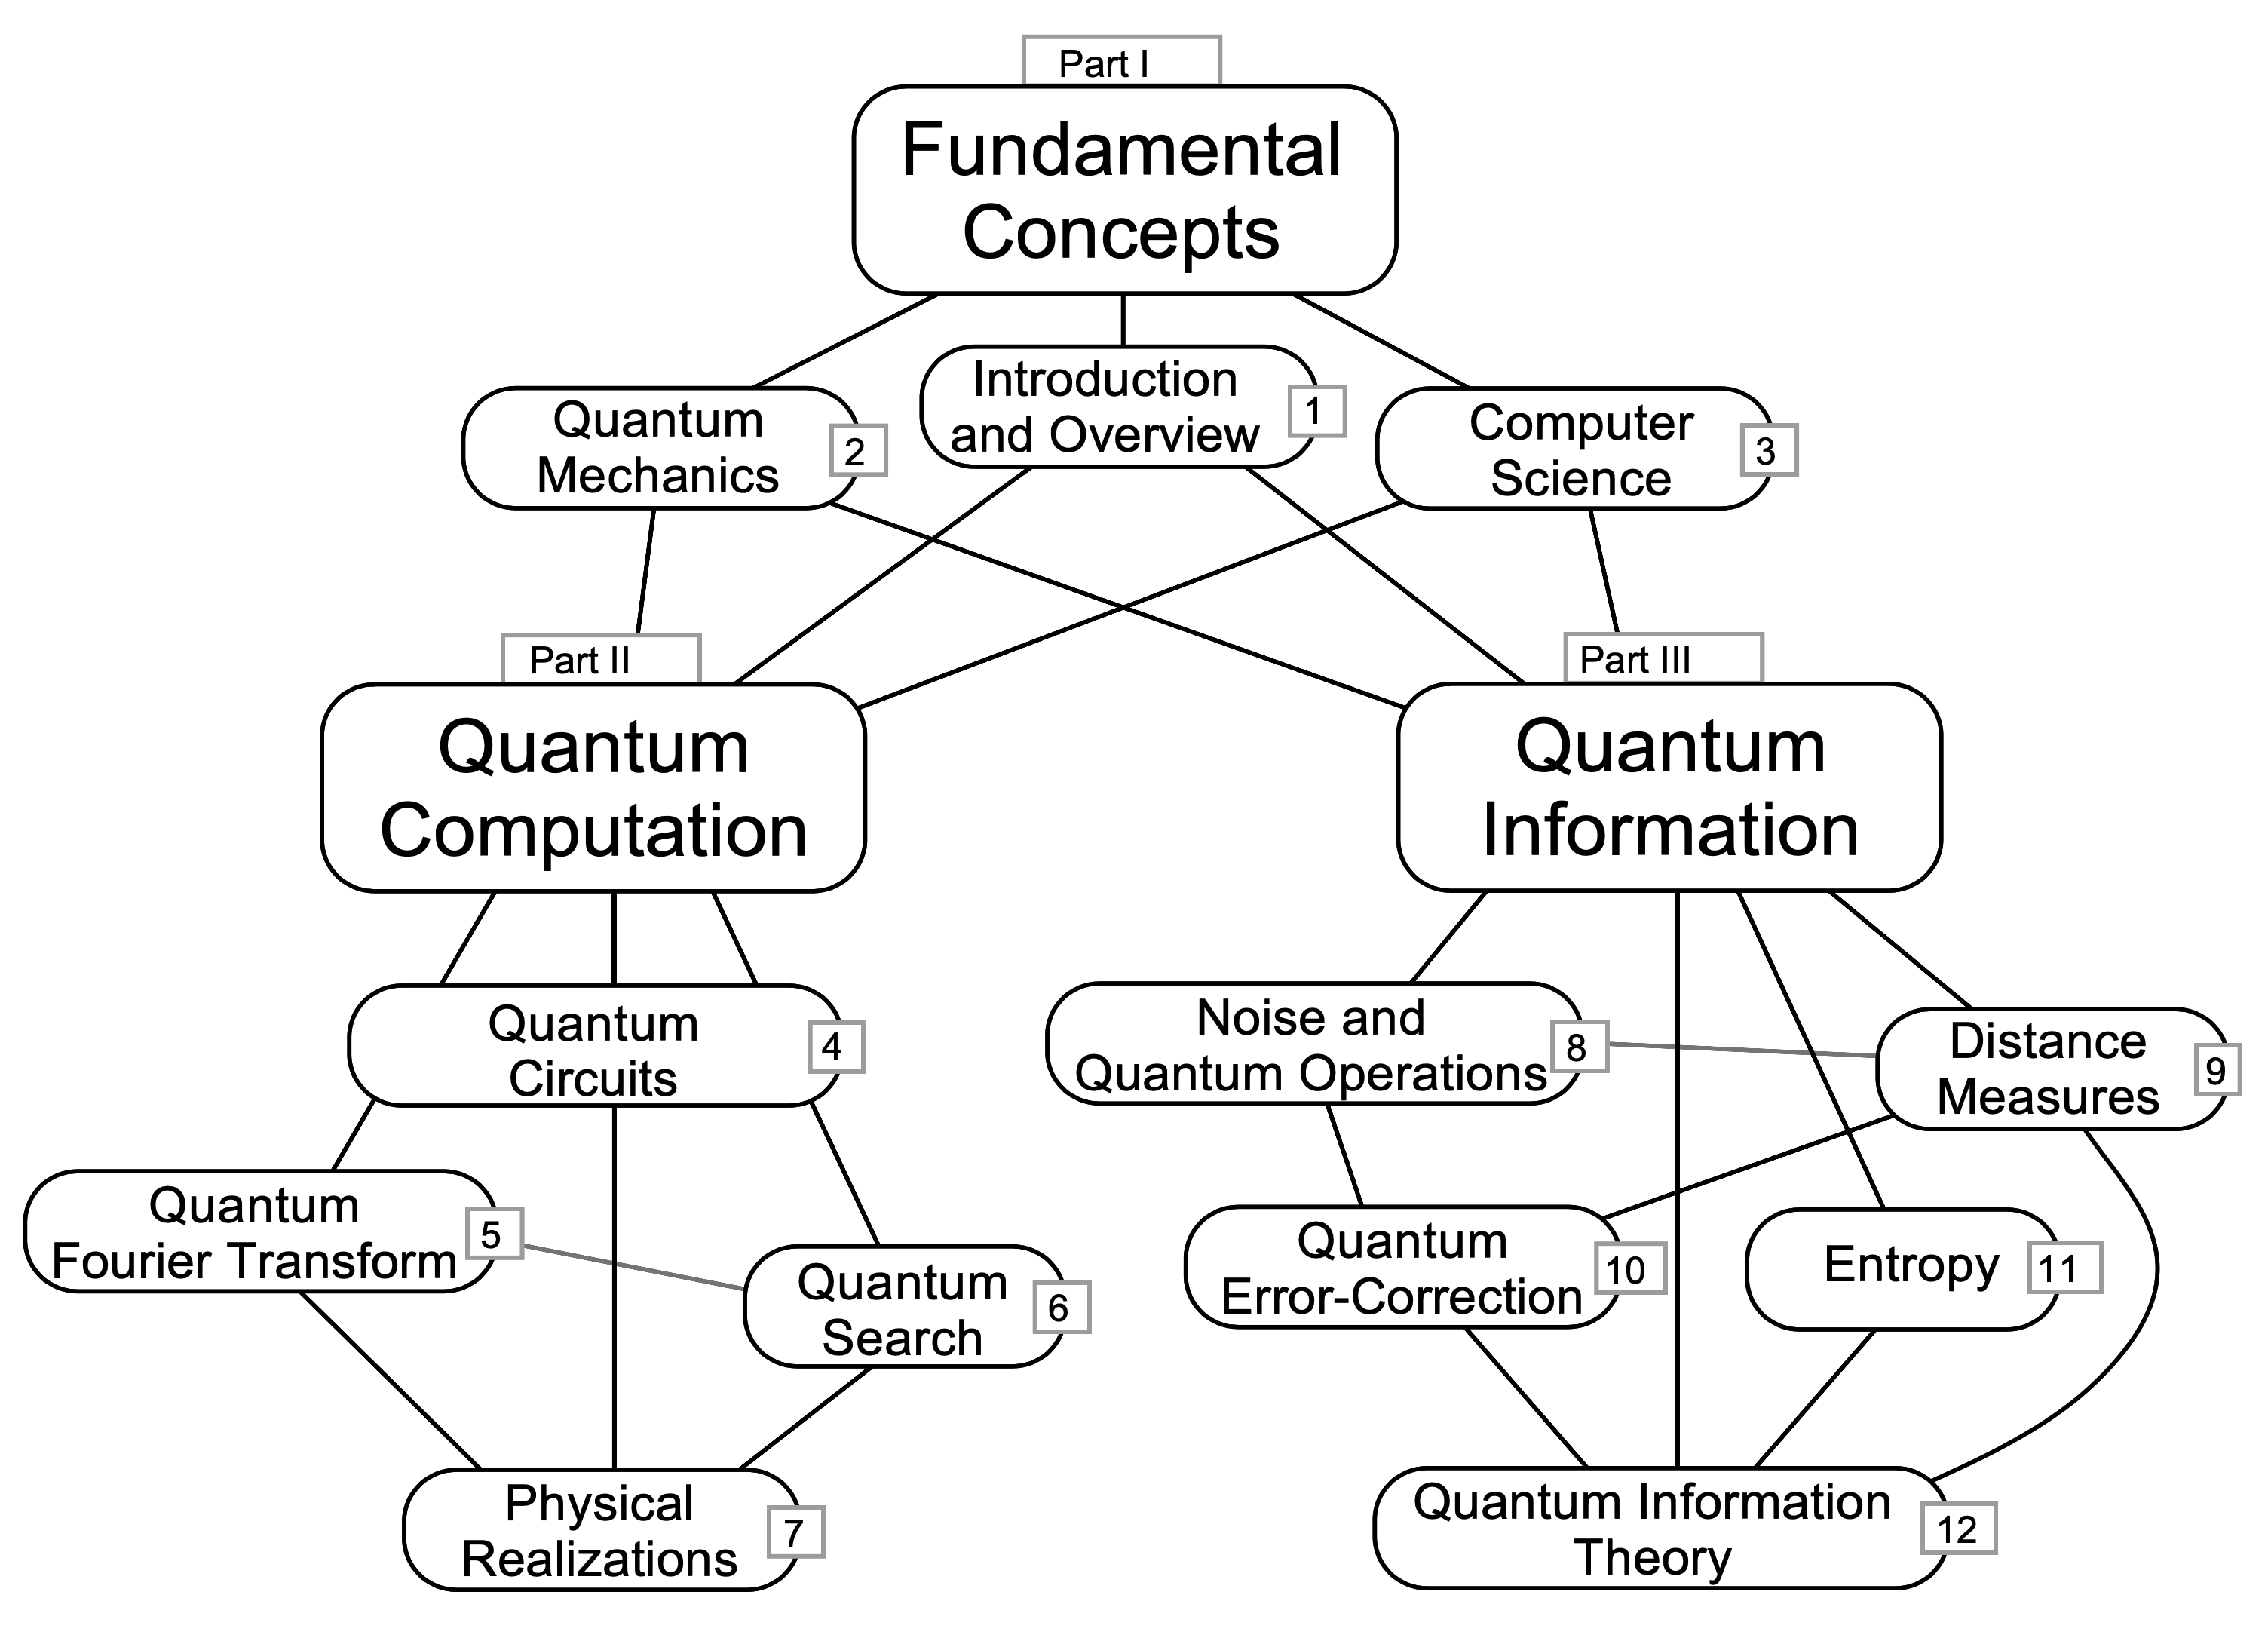
\includegraphics[width=\textwidth]{category.png}
  \caption{A big picture for the quantum computation and 
  quantum information field in Issac Chuang's book. The proposal 
  here focuses more on quantum circuits and quantum fourier transform study. }
\end{figure}

\subsection*{Quantum Gates, Quantum Circuit, and Quantum Computation}
Clasical computer consists of wires and logic gates. Similarly, 
the quantum computer takes quantum version and logic gates and act on 
each qubit. The most famous Pauli Matrices, X are used as NOT gates: 
\begin{equation}
  X = \begin{bmatrix}
    0 & 1 \\ 1 & 0 
  \end{bmatrix},
  Y = \begin{bmatrix}
    0 & -i \\ i & 0 
  \end{bmatrix},
  Z = \begin{bmatrix}
    1 & 0 \\ 0 & -1 
  \end{bmatrix}
\end{equation}
Z gate flips the sign of $\ket{1}$ to give $-\ket{1}$ and 
\textit{Hadamard} gate, 
\begin{equation}
  H =  \frac{1}{\sqrt{2}}\begin{bmatrix}
    1 & 1 \\ 1 & -1
  \end{bmatrix}, S = \begin{bmatrix}
    1 & 0 \\ 0 & i
  \end{bmatrix}, T = \begin{bmatrix}
    1 & 0 \\ 0 & exp(i \pi/4)
  \end{bmatrix}
\end{equation}
Hadamard gate turns $\ket{0}$ into $(\ket{0}+\ket{1})/\sqrt{2}$, and 
$\ket{1}$ into $(\ket{0}-\ket{1})/\sqrt{2}$, phase gate S and $\pi/8$ gate T 
have some algebraic relation with H that $H = (X+Z)/\sqrt{2}$ and 
$S = T^2$. For rotation matrix around X, Y, Z, rotates around x, y, z axes, 
they are defined by equation:
$$R_{\eta}(\theta) = e^{-i \theta \eta /2} = \cos \frac{\theta}{2}I -i \sin \frac{\theta}{2} \eta, \ \ \ \eta \in \{X,Y,Z\}$$
Some important theorem likes Z-Y decomposition for a single qubit 
exits. Suppose U is a unitary operation on a single qubit. Then there exist
real numbers $\alpha, \beta, \gamma, \delta$ such that 
\begin{equation}
  U = e^{i \alpha} R_z(\beta) R_y (\gamma) R_z(\delta)
\end{equation}

\subsubsection*{Controlled Operations}
Here are some controlled openeration with CNOT gate. The core 
idea for controlled operation is "If A is true, then do B". On 
single qubit, in terms of the computational basis, the action
of the CNOT is given by $\ket{c} \ket{t} \rightarrow \ket{c} \ket{t \bigoplus c }$,
which means that the control qubit is set to $\ket{1}$ then the target
qubit is flipped, otherwise the target qubit is left alone. Thus, 
in the computational basis $\ket{control, target}$ the matrix representation
of CNOT is: 
\begin{equation}
  \begin{bmatrix}
    1 & 0 & 0 & 0 \\
    0 & 1 & 0 & 0 \\
    0 & 0 & 0 & 1 \\
    0 & 0 & 1 & 0 
  \end{bmatrix}
\end{equation}
which could also replace by \textit{controlled-U} operation. 
\begin{figure}[h]
  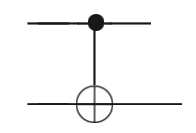
\includegraphics[width=0.20\textwidth]{cnot.png}
  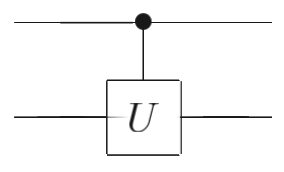
\includegraphics[width=0.24\textwidth]{cnot-u.png}
  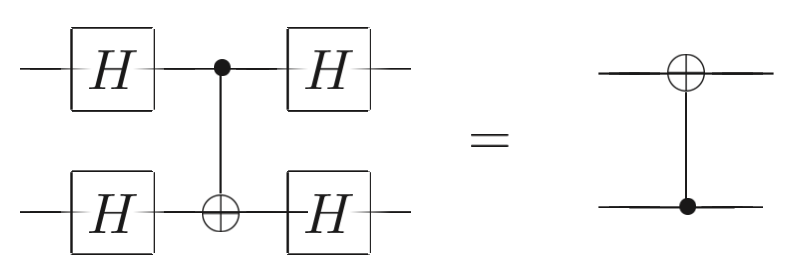
\includegraphics[width=0.48\textwidth]{cnot-h.png}
  \caption{Some circuit representation of control operation}
\end{figure}
\subsection*{Encoding Classical Data into Quantum States}
Quantum Encoding is a process to transform classical information into quantum 
states. In order to use quantum algorithms to solve classical problems, 
such encoding is unavoidable. The simple concept is quantum circuit acts on 
$\ket{0^n}$ state, where n is the number of qubits. Based on different 
requirements, the style of requirement is different. The first three are 
most basic ones and the last two require more depth. 

\subsubsection*{Basis Encoding}
Conceptually the simplest one, encodes an n-bit binary string to an n-qubit 
quantum state $\ket{x} = \ket{i_x}$, where $\ket{i_x}$ is a computational
basis state. Concrete example: $ x =1011 $ maps to $\ket{1011}$

\subsubsection*{Amplitude Encoding}
Vector $x$ of length $N$ into amplitudes of an n-qubit quantum 
state with $n = [log_2(N)]$ and $
  \ket{x} = \sum^N_i x_i \ket{i} $
and $\ket{i}$ is the computational basisi for the Hilbert space. Since 
the classical information forms the amplitudes of a quantum state, the 
input needs to satisfy the normalization condition. For instance, 
$x1 = \begin{bmatrix}
  1/2 \\ 1/2 \\ -1/2 \\-1/2
\end{bmatrix}$, the quantum state will be written as: 
$\ket{x1} = \frac{1}{2} \ket{00} + \frac{1}{2} 
\ket{01} - \frac{1}{2} \ket{10} - \frac{1}{2} \ket{11}$
similarly, for $x2 = \begin{bmatrix}
  1/\sqrt{3} \\ 1/\sqrt{3} \\ -1/\sqrt{3} 
\end{bmatrix}$ the state would be:
$\ket{x2} = \frac{1}{\sqrt{3}} \ket{00} 
+ \frac{1}{\sqrt{3}} \ket{01} - \frac{1}{\sqrt{3}} \ket{10} $

\subsubsection*{Angle Encoding}
Angle encoding uses rotation gates to encode the classical information x. 
The classical information determines angles of rotation gates:
\begin{equation}
  \ket{x} = \bigotimes_i^n R(x_i) \ket{0^n}
\end{equation}
R can be one of the rotation gate $R_x$, $R_y$, and $R_z$. Usually, the 
number of qubits used for enoding is equal to the dimension of vector. For example, 
if $x = \begin{bmatrix}
  \pi \\ \pi \\ \pi 
\end{bmatrix}$, angle encoding rotates every qubit around Y-axis (if we choose $R_y$)
for degree $\pi$, the corresponding quantum state is then $\ket{x} = Ry(\pi) \ket{0} Ry(\pi) \ket{0} Ry(\pi) \ket{0}$
, which indicates the result is $\ket{111}$.

\subsubsection*{IQP Style Encoding}

\subsubsection*{Hamiltonian Evolution Ansatz Encoding}

\subsection*{Quantum Classifier}

\begin{figure}[h]
  \begin{center}
    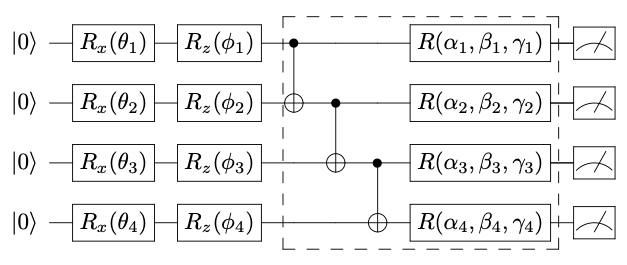
\includegraphics[width=0.58\textwidth]{vqc.png} 
    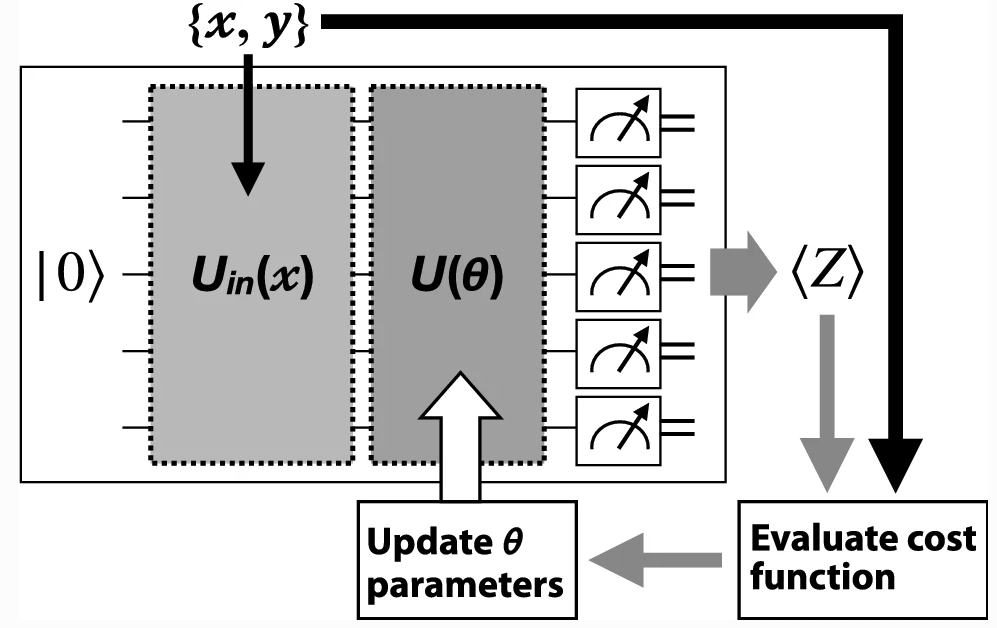
\includegraphics[width=0.38\textwidth]{vqc1.png} 
  \end{center}
  \caption{The generic variational quantum circuit 
  architecture and procedure for optimization. The 
  inputs go through encoding, the unitary matrices, 
  measurement, lost function evalution and then 
  update parameters.}
\end{figure}

The lost function could be the simplest one: 
\begin{equation}
  L (\theta) = \sum^N_{k=1} \frac{1}{N} |\tilde{y}^k - y^k|^2
\end{equation}
\subsection*{Quantum Fourier Transform Phase Estimation}
Suppose a unitary operator U has an eigenvalue $\ket{u}$ with 
eigenvalue $e^{2 \pi i \varphi}$, where the value of 
$\varphi$ is unknown. The goal of the 
phase estimation algorithm is to estimate $\varphi$.
\newline
\textbf{Inputs:} (1) A black box which performs a 
controlled-$U^j$ operation, for integer j. (2) an 
eigenstate $\ket{u}$ of U with eigenvalue $e^{2 \pi i \varphi}$, and 
(3) $t = n + [log(2+\frac{1}{2 \epsilon})]$ qubits initialized 
to $\ket{0}$ \newline
\textbf{Outputs:} An n-bit approximation $\tilde{\varphi_u}$ to $\varphi_u$ \newline
\textbf{Runtime:} $O(t^2)$ operations and one call to controlled-$U^j$
black box. Succeeds with probability at least $1-\epsilon$. \newline
\textbf{Procedure}: 
\begin{enumerate}
  \item $\ket{0}\ket{u}$  initial state
  \item $\rightarrow \frac{1}{\sqrt{2^t}} \sum^{2^t -1}_{j=0} \ket{j}\ket{u} $ create superposition
  \item $\rightarrow \frac{1}{\sqrt{2^t}} \sum^{2^t -1}_{j=0} \ket{j} U^j \ket{u} $ apply black box
  \item $= \frac{1}{\sqrt{2^t}} \sum^{2^t -1}_{j=0}  e^{2 \pi i j \varphi_u} \ket{j} \ket{u} $ result of black box 
  \item $\rightarrow \ket{\tilde{\varphi_u}} \ket{u}$
  \item  $\rightarrow \tilde{\varphi_u}$
\end{enumerate}

\subsection*{Quantum Fourier Transform Shor's Algorithm}


\textbf{References on Riemannian Manifold related research:}
\begin{enumerate}
  \item Slavakis Lab: \href{https://ieeexplore.ieee.org/document/9321498}{Fast Sequential Clustering in Riemannian Manifolds 
  for Dynamic and Time-Series-Annotated Multilayer Networks}
  \item Slavakis Lab: \href{https://ieeexplore.ieee.org/document/9699419}{Kernel Regression Imputation in Manifolds Via Bi-Linear Modeling: 
  The Dynamic-MRI Case}
\end{enumerate}

\textbf{References on Quantum Machine Learning: Quantum Kernel Methods}
\begin{enumerate}
  \item Maria Schuld: \href{https://arxiv.org/abs/2101.11020}{Supervised quantum machine learning models are kernel methods}
  \item IBM T.J. Watson Research Center: \href{https://arxiv.org/abs/1804.11326}{Supervised learning with quantum enhanced feature spaces}
  \item Yunchao Liu, IBM Quantum: \href{https://arxiv.org/abs/2010.02174}{A rigorous and robust quantum speed-up in supervised machine learning}
  \item Maria Schuld: \href{https://arxiv.org/abs/1803.07128}{Quantum machine learning in feature Hilbert spaces}
  \item Thomas Hubregtsen: \href{https://arxiv.org/abs/2105.02276}{Training Quantum Embedding Kernels on Near-Term Quantum Computers}
  \item Online Python Lib: \href{https://qiskit.org/documentation/machine-learning/tutorials/03_quantum_kernel.html
  }{Qiskit Link}
  \item Online Python Lib: \href{https://pennylane.ai/qml/demos/tutorial_kernel_based_training.html}{Pennylane}
\end{enumerate}

\textbf{References on Quantum Machine Learning Application}
\begin{enumerate}
  \item Wen Guan et al: \href{https://iopscience.iop.org/article/10.1088/2632-2153/abc17d}{
    Quantum machine learning in high energy physics}
  \item Wonho Jang et al: \href{https://arxiv.org/abs/2102.10008}{
    Quantum Gate Pattern Recognition and Circuit Optimization for Scientific Applications}
  \item Koji Terashi et al:\href{https://link.springer.com/article/10.1007/s41781-020-00047-7}{Event Classification 
  with Quantum Machine Learning in High-Energy Physics }
\end{enumerate}

\textbf{References on Quantum Signal Processing: Quantum Fourier Transform}
\begin{enumerate}
  \item Nielson and Chuang: Quantum Computation and Quantum Information
  \item Peter Shor: \href{https://www.cl.cam.ac.uk/teaching/1920/QuantComp/Quantum_Computing_Lecture_9.pdf}{Lecture on Quantum Computing
  and quantum Fourier transforms}
  \item Shor's Algorithm \href{https://en.wikipedia.org/wiki/Shor%27s_algorithm}{wiki} \href{https://quantum-computing.ibm.com/composer/docs/iqx/guide/shors-algorithm}{IBM quantum composer} 
  \item Leandro Aolita et. al: \href{https://arxiv.org/abs/2206.02826}{Fourier-based quantum signal processing}
  \item Alok Anand et. al: \href{https://arxiv.org/pdf/2203.01831.pdf}{Quantum Image Processing }
  \item Qiskit: \href{https://qiskit.org/textbook/ch-applications/image-processing-frqi-neqr.html}{Quantum Image Processing}
\end{enumerate}

\textbf{References on Quantum Signal Processing: Encoding Theory }
\begin{enumerate}
  \item Marcello Benedetti et. al: \href{https://iopscience.iop.org/article/10.1088/2058-9565/ab4eb5}{Parameterized quantum circuits as machine learning models
  }
\end{enumerate}

\textbf{References}
\begin{enumerate}
  \item Hamiltonian Evolution Ansatz Encoding: \href{https://journals.aps.org/prb/abstract/10.1103/PhysRevB.102.235122}{Strategies for solving the Fermi-Hubbard model on near-term quantum computers}
\end{enumerate}




% Overall view of the research proposal 
% Interviewer 
% Will your master transfer 
% How to encode 
% There are 

% What will be the things other than encoding?
% How to run the algorithm if Quantum Computer not 
% New idea on signal processing? Doing the translation is 
% bring the novelty part to the front. 
% Avoid doing the implementation 

% Highlight the major contribution of the proposal
% 15minutes Slides: present the main idea 
% giving people some impression. 

% Heat Kernel or Diffusion Kernel. Typical Machine 
% Learning Stuff. 

% Restructure the research proposal: 
% Don't have idea of what quantum machanic is. 
% A single slide for people understand how 
% quantum state: resembles with machine learning. 
% Keep the flow 
% They may have problems with technical issues. 
% How my project will contribute a lot for the 
% field. 
% How we know things? How we know to bring the games 
% into the
% We don't have quantum computer here. 
% How I going to test algorithms: 
% emulation on super computer. more funding. 
% some example: Pixel and image. 

% You can image one in the Linear vector space. 
% explain things in engineering department's view. 
% Audience are different people. 
% Why would you like to come to engineering department? 
% Novel contribution to the signal processing field?
% What are the novel things in Quantum Machine Learning? 
% 

\section{Present Field of Study}

The pixel hit information plays vital rule for the charge particle track reconstructions,
especially for flavor tagging such as c-, b-quark jets or hadronic tau identifications, where
they form as a colimated spray of the charged particles. The track reconstruction software
has been developed to identify such particles in the dense environment of the very narrow
space using the neural network technique. Meanwhile, the pixel detector has been experienced
significant radiation damage that degradates the performance. The pixel hits will be lost at
most 50\% of efficiency in b-layer in the end of RUN3, in turn lost the performance for the
cluster classification to split or merge the associated cluster in the dense track reconstruction.
The evaluation of the radiation damage of the pixel detector and modeling of the pixel cluster
classification in the simulation is thus critical to improve the systematic uncertainties through
RUN3.
The task devotes to monitor the pixel cluster classification performance using the
$Z \rightarrow \tau \tau$ events. The hadronic tau with 3-prong decay mode is a clean source for the dense
tracking. The task first constructs clean dataset of the $Z \rightarrow \tau \tau$ with 3-prong final state, then
the pixel clustering is compared with the simulation in a various view in term of the radiation
damage. The produced dataset would be useful for many area for the tracking aspect as further
optimization of the neural network training \cite{pixel}.

\newpage